%
% File acl2019.tex
%
%% Based on the style files for ACL 2018, NAACL 2018/19, which were
%% Based on the style files for ACL-2015, with some improvements
%%  taken from the NAACL-2016 style
%% Based on the style files for ACL-2014, which were, in turn,
%% based on ACL-2013, ACL-2012, ACL-2011, ACL-2010, ACL-IJCNLP-2009,
%% EACL-2009, IJCNLP-2008...
%% Based on the style files for EACL 2006 by 
%%e.agirre@ehu.es or Sergi.Balari@uab.es
%% and that of ACL 08 by Joakim Nivre and Noah Smith

\documentclass[11pt,a4paper]{article}
\usepackage{authblk}
\usepackage[hyperref]{acl2019}
\usepackage{times}
\usepackage{latexsym}
\usepackage{graphicx}
\usepackage{multirow}
\usepackage{enumitem}
\usepackage{url}
\usepackage{tcolorbox}
\usepackage{bbold}
\usepackage{amsmath}

\newcommand{\subscript}[2]{$#1#2$}

\aclfinalcopy % Uncomment this line for the final submission
%\def\aclpaperid{***} %  Enter the acl Paper ID here

%\setlength\titlebox{5cm}
% You can expand the titlebox if you need extra space
% to show all the authors. Please do not make the titlebox
% smaller than 5cm (the original size); we will check this
% in the camera-ready version and ask you to change it back.

\newcommand\BibTeX{B\textsc{ib}\TeX}
\DeclareRobustCommand{\VAN}[3]{#2} % set up for citation

\title{Detecting Argumentative Discourse Acts with Linguistic Alignment}

\author{\textbf{Timothy Niven}}
\author{\textbf{Hung-Yu Kao}}
\affil{Intelligent Knowledge Management Lab \\
  Department of Computer Science and Information Engineering \\
  National Cheng Kung University \\
  Tainan, Taiwan \\
  \texttt{tim.niven.public@gmail.com}, \texttt{hykao@mail.ncku.edu.tw}}

\date{}

\begin{document}
\maketitle
\begin{abstract}
  We report the results of preliminary investigations into the relationship between linguistic alignment and dialogical argumentation at the level of discourse acts. We annotated a proof of concept dataset with illocutions and transitions at the comment level based on Inference Anchoring Theory. We estimated linguistic alignment across discourse acts and found significant variation. Alignment features calculated at the dyad level are found to be useful for detecting a range of argumentative discourse acts.
\end{abstract}

%
% Introduction

\section{Introduction}

Argumentation mining remains a difficult problem for machines. Even for humans, understanding the substance of an argument can involve complex pragmatic interpretation \cite{Cohen87}. Consider the reply of \textit{B} in Figure 1. Absent broader conversational context, and perhaps knowledge of the background beliefs of \textit{B}, it can be difficult to judge whether they are asking ``which religions are correlated with increased life expectancy?'' (pure questioning) or giving their opinion that ``not just any religion is correlated with a longer life'' (assertive questioning). Since only the latter is an argumentative discourse unit (ADU) \cite{Stede13}, ambiguities like this therefore make it difficult to accurately identify the structure of argumentation.

In this work we investigate using a subtle yet robust signal to resolve such ambiguity: linguistic alignment. Alignment can be calculated in an unsupervised manner and does not require textual understanding. It is therefore well suited to our current technology as an extra pragmatic feature to assist dialogical argumentation mining. Our hypothesis is that, since alignment has been shown to relate to communication strategies \cite{DoyleF16}, different alignment effects will be observed over different argumentative discourse acts, providing signal for their detection. For example, Figure 2 shows our estimated posterior densities for alignment scores over pure and assertive questioning. On this basis, if \textit{B}'s comment in Figure 1 is accompanied by a significantly positive alignment score, we would be correct more often than not classifying it as assertive questioning.

\begin{figure}[t]
\small
$\mathbf{A}$: ...To be able to claim that life expectancy and health are tied to religion you have to rule out hundreds of other factors: diet; lifestyle; racial characteristics; genetic pre-disposition (religion tends to run in families) etc...

\vspace{6pt}

$\mathbf{B}$: ...Can I just have ANY religion and have a longer life?
\caption{An example dyad from our dataset. Without disambiguating information it is hard to know if B's reply is pure or assertive questioning.}
\end{figure}

\begin{figure}[t]
\centering
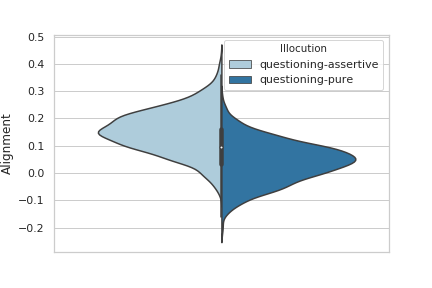
\includegraphics[width=0.45\textwidth]{compare_dists.png}
\caption{Posterior densities on alignment estimates for pure and assertive questioning in our dataset, indicating that alignment can help to disambiguate discourse acts.}
\end{figure}

In this preliminary work we aim to address the following questions:

\begin{enumerate}
    \item Are the majority of argumentative discourse acts associated with significantly different alignment effects?
    \item Are alignment features useful for detecting argumentative discourse acts?
\end{enumerate}

\section{Background and Related Work}

Linguistic alignment is a form of communication accommodation \cite{GilesCC91} whereby speakers adapt their word choice to match their interlocutor \cite{NiederhofferP02}. It can be calculated as an increase in the probability of using a word category having just heard it, relative to a baseline usage rate. An example is given in Figure 3. Note that alignment is calculated over \textit{non-content} word categories.\footnote{Previous work has indicated the primacy of word-based over category-based alignment \cite{DoyleF16}. We leave investigation of alignment over words in argumentation to future work.} While content words are clearly set by the topic of conversation, the usage rates of particular non-content word categories has shown to be a robust measure of linguistic style \cite{PennebakerK00}. Consistent with previous work, we focus on alignment over the Linguistic Inquiry and Word Count (LIWC) categories \cite{PennebakerBJB15}, listed in Table 1.

Linguistic alignment is a robust phenomenon found in a variety of settings. It has been used to predict employment outcomes \cite{SrivastavaGMP18}, romantic matches \cite{IrelandSESFP}, and performance at cooperative tasks \cite{FusaroliBORRFT12, KacewiczPDJG14}. People have been found to align to power \cite{WillemynsGCP97, Gnisci05, DanescuLPK11}, to people they like \cite{BilousK88, Natale75}, to in-group members \cite{ShinD18}, and to people more central in social networks \cite{NobleF15}. The variety of these contexts suggest alignment is ubiquitous and modulated by a complex range of factors.

Some previous work bears on argumentation. Binarized alignment features indicating the presence of words from LIWC categories were found to improve the detection of disagreement in online comments \cite{RosenthalM15}. We utilize more robust calculation methods that account for baseline usage rates which thereby avoid mistaking similarity for alignment \cite{DoyleYF16}. Accommodation of \textit{body movements} was found to decrease in face-to-face argumentative conflict where interlocutors had fundamentally differing opinions \cite{PaxtonD13, DuranF17}. In contrast we are concerned with linguistic forms of alignment.

\begin{figure}[t]
\begin{center}
\small
\begin{tabular}{|c|cc|}
\hline
\multirow{2}{*}{} & \multicolumn{2}{c|}{B's reply} \\
A's message & has pronoun & no pronoun \\
\hline
has pronoun & 8 & 2 \\
no pronoun & 5 & 5\\
\hline
\end{tabular}
\end{center}
\caption{Example of linguistic alignment using a binarized ``by-message'' calculation technique \cite{DoyleF16}. \textit{B}'s baseline usage rate of pronouns is $0.5$, coming from the bottom row. The top row shows the probability of \textit{B} using a pronoun increases to $0.8$ after seeing one in \textit{A}'s message.}
\end{figure}

\begin{table}[t]
\begin{center}
\small
\begin{tabular}{|c|c|c|}
\hline
Category & Examples & Usage \\
\hline
Article & \textit{a, the} & 0.076 \\
Certainty & \textit{always, never} & 0.016 \\
Conjunction & \textit{but, and, though} & 0.060 \\
Discrepancy & \textit{should, would} & 0.018 \\
Negation & \textit{not, never} & 0.018 \\
Preposition & \textit{to, in, by, from} & 0.137 \\
Pronoun & \textit{it, you} & 0.108 \\
Quantifier & \textit{few, many} & 0.025 \\
Tentative & \textit{maybe, perhaps} & 0.030 \\
Insight & \textit{think, know, consider} & 0.027 \\
Causation & \textit{because, effect, hence} & 0.021 \\
\hline
\end{tabular}
\end{center}
\caption{LIWC dictionary categories we use, examples, and baseline production rates observed in our dataset of $\sim1.5$ million comments on news articles.}
\end{table}

We focus on the argumentative discourse acts of Inference Anchoring Theory (IAT) \cite{BudzynskaR11, BudzynskaJRS16}. IAT is well motivated theoretically, providing a principled way to relate dialogue to argument structure. As noted above, an utterance that has the surface form of a question may have different functions in an argument - asking for a reason, stating a belief, or both. The IAT framework is designed to make these crucial distinctions, and covers a comprehensive range of argumentative discourse acts.

\begin{figure*}[t]
\centering
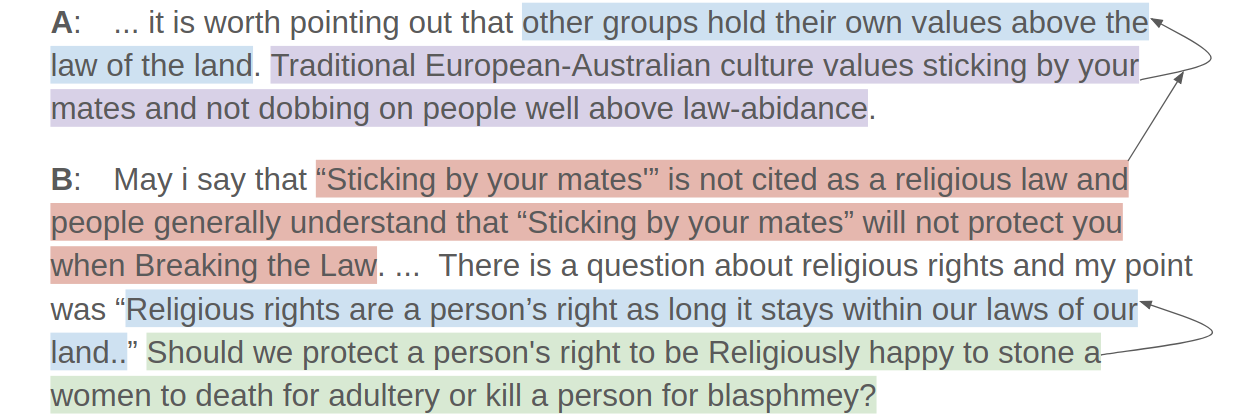
\includegraphics[width=0.8\textwidth]{annotate.png}
\caption{Annotating discourse acts across a message-reply pair. The blue text spans are \textit{Asserting}. The red span is \textit{Disagreeing}, which always crosses the comments - in this case attacking the inference in \textit{A}. If \textit{A} was the reply we would annotate the purple span as \textit{Arguing}, as it offers a reason in support of the preceding assertion. In the reply, \textit{Arguing} is provided by the green span, which is an instance of \textit{Assertive Questioning}. Note that we only annotate what is in \textit{B}. This pair is therefore annotated as: \{\textit{Asserting}, \textit{Disagreeing},  \textit{Assertive Questioning}, \textit{Arguing}\}.}
\end{figure*}

Two previous datasets are similar to ours. The US 2016 Election Reddit corpus \cite{VisserKDKBR19} comes from our target genre and is reliably annotated with IAT conventions. However, the content is restricted to a single topic. Furthermore, political group effects have already been demonstrated to influence alignment \cite{ShinD18}. These considerations limit our ability to generalize using this dataset alone. The Internet Argument Corpus \cite{AbbottEAW16}, used in prior work on disagreement \cite{RosenthalM15}, is much larger than our current dataset, however the annotations do not cover the principled and comprehensive set of discourse acts that we require to support dialogical argumentation mining in general.

%
% Dataset

\section{Dataset}

In this section we outline our annotation process. So far we have $800$ message-reply pairs but annotated by just a single annotator. In future work we will scale up considerably with multiple annotators, and include Mandarin data for cross-linguistic comparison.

\subsection{Source}

We scraped $\sim$1.5M below the line comments from an academic news website, The Conversation,\footnote{\hyperlink{https://theconversation.com/global}{https://theconversation.com/global}} covering all articles from its inception in 2011 to the end of 2017. In order to maximize the generalizabilty of our conclusions we selected comments covering a variety of topics. We also picked as evenly as possible from the continuum of controversiality, as measured by the proportion of deleted comments in each topic. More controversial topics are likely to see higher degrees of polarization, which should affect alignment across groups \cite{ShinD18}. The most controversial topics we included are \textit{climate change} and \textit{immigration}. Among the least controversial are \textit{agriculture} and \textit{tax}.

Nevertheless this data source has its own peculiarities that attenuate liberal generalization. As the site is well moderated, comments are on topic and abusive comments are deleted, even if they also contain argumentative content. The messages are generally longer and less noisy than, for example, Twitter data. Moreover, many commenters are from research and academia. Therefore in general we see a high quality of writing, and of argumentation.

% Since alignment effects are sensitive to social group effects \cite{ShinD18} we wanted to avoid unevenly focusing on highly controversial topics that see high degrees of polarization. In our annotations we therefore aimed for an even distribution over degrees controversy over topics. We used the ratio of deleted over total comments under each topic as a proxy for controversy and selected topics from all over this spectrum. Figure 4 shows the distribution of degree of controversy over the message-reply pairs we annotated. If anything our current distribution is skewed towards less controversy, but this distribution does reflect the natural distribution in the data. MAYBE I CAN JUST DROP THIS POINT.

% \begin{figure}[t]
% \centering
% 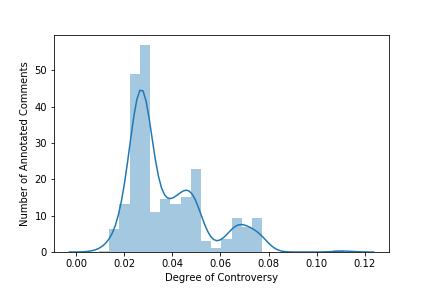
\includegraphics[width=0.45\textwidth]{controversy.png}
% \caption{XXX.}
% \end{figure}

\subsection{Annotation}

The list of illocutions we chose to annotate are taken from \citeauthor{BudzynskaJRS16} \shortcite{BudzynskaJRS16}: \textit{Asserting}, \textit{Ironic Asserting}, \textit{(Pure/Assertive/Rhetorical) Questioning}, \textit{(Pure/Assertive/Rhetorical) Challenging}, \textit{Conceding}, \textit{Restating}, and \textit{Non-Argumentative} (anything else). The transitions we consider follow IAT conventions. \textit{Arguing} holds over two units, where a reason is offered as support for some proposition. \textit{Disagreeing} occurs where an assertion conflicts with another. \textit{Agreeing} is instantiated by phrases such as ``I agree'' and ``Yeah.''

Annotating \textit{Rhetorical}  \textit{Questioning/Challenging} is the most difficult. As noted by  \citeauthor{BudzynskaJRS16} \shortcite{BudzynskaJRS16}, there is no common specification for \textit{Rhetorical Questioning}. We follow their definition, by which \textit{Pure} and \textit{Assertive Questioning/Challenging} ask for the speaker's opinion/evidence, and the \textit{Assertive} and \textit{Rhetorical} types communicate the speakers own opinion. Therefore the \textit{Pure} varieties do not convey the speakers opinion, and the \textit{Rhetorical} types do not expect a reply. Annotating \textit{Rhetorical Questioning/Challenging} therefore requires a more complicated pragmatic judgment of the speaker's intention.

Our annotation scheme departs from previous work in that we only annotate at the comment and not the text segment level. Multiple annotations often apply to a single comment. An example is given in Figure 4. The text spans of the identified illocutions are highlighted and the transitions are indicated with arrows for clarity, but note that we did not annotate at that level.

Another difference from prior work relates to \textit{Concessions}. Unlike \citeauthor{BudzynskaJRS16} \shortcite{BudzynskaJRS16} we do not explicitly annotate the sub-type \textit{Popular Concession} - where a speaker concedes in order to prepare the ground for disagreement. A potential confound with the annotation scheme described so far is ambiguous cases of \textit{Agreeing} and \textit{Disagreeing} in the same comment, which could be expected in a \textit{Popular Concession}: ``Yeah, I agree that X, but [counter-argument].'' Because we are annotating at the level of the comment, we are able to distinguish these cases by considering combinations of discourse acts. A \textit{Popular Concession} is distinguished by the presence of \textit{Conceding} along with \textit{Disagreeing}, optionally with \textit{Agreeing}. A \textit{Pure Concession} is then distinguished by the presence of \textit{Conceding} and the absence of \textit{Disagreeing}. We therefore do not need to rule that only one of \textit{Agreeing} or \textit{Disagreeing} can occur in a single comment.

We found that \textit{Asserting} (627/800), \textit{Arguing} (463/800), and \textit{Disagreeing} (402/800) are by far the most common individually, and as a combination (339/800), reflecting the argumentative nature of our dataset. The distribution of comments over discourse acts is Zipfian. The lowest frequency discourse act is \textit{Ironic Asserting}, which has only 12 annotations in our 800 comments.

%
% Methodology

\section{Methodology}

\subsection{Alignment over Discourse Acts}

To estimate alignment scores across discourse acts we parameterize the message and reply generation process as a hierarchy of normal distributions, following the word-based hierarchical alignment model (WHAM) \cite{DoyleF16}. Each message is treated as a bag of words and word category usage is modeled as a binomial draw. WHAM is based on the hierarchical alignment model (HAM) \cite{DoyleYF16}, adapted by much other previous work \cite{DoyleF16, YurovskyDF16, DoyleGSF17}. WHAM's principal benefit over HAM is controlling for message length, which was shown to be important for accurate alignment calculation \cite{DoyleF16}. Our adaptation is shown in Figure 5. For further details of WHAM we refer the reader to the original work.

\begin{figure}[t]
\centering
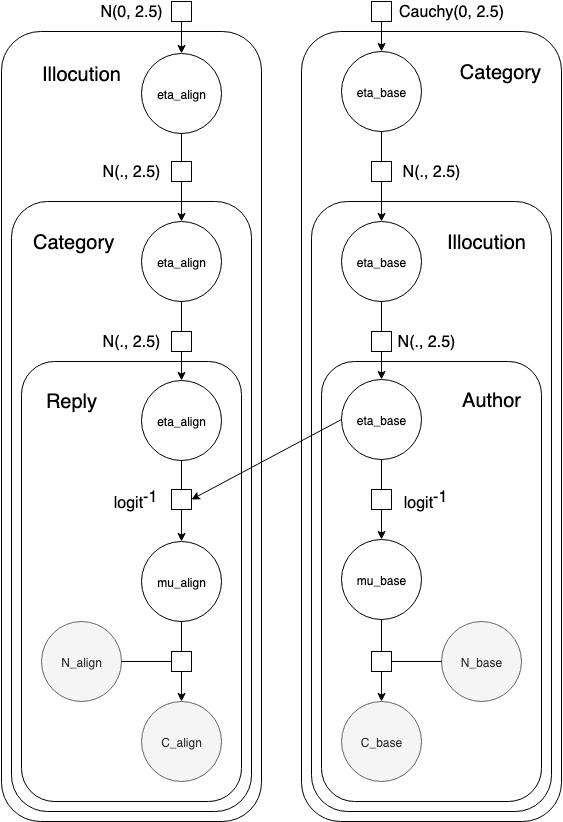
\includegraphics[width=0.45\textwidth]{MyHAM.png}
\caption{Our adaptation of WHAM \cite{DoyleF16} for estimating alignment over argumentative discourse acts.}
\end{figure}

A key problem we need to address is our inability to aggregate counts over all messages in a conversation between two speakers (as in Figure 3). This is a virtue of the original WHAM model that provides more reliable alignment statistics. We cannot aggregate counts over multiple message-reply pairs since our target is the discourse acts in \textit{individual} replies. However, we are helped somewhat by the long average comment length in our chosen genre ($\mu = 82.5$ words, $\sigma = 66.5$). The lowest baseline category usage rate is approximately $0.8\%$ ($\mu = 3.6\%$, $\sigma = 2.2\%$). Therefore an average comment length gives us enough opportunity to see much of the effects of alignment on the binomial draw, but is likely to systematically underestimate alignment. In future work we will investigate this phenomenon with simulated data, and continue to search for a solution that makes better use of the statistics.

However, we can make more robust estimates of the baseline rate of word category usage by considering our entire dataset ($\sim 1.5$ million comments). We have annotations for $261$ authors. The most prolific author has $11,327$ comments. On average an author has $429$ comments ($\sigma = 1,409$). For most authors we find multiple replies to comments that do not have each word category, making these statistics relatively reliable.

Bayesian posteriors for discourse act alignments are then estimated using Hamiltonian Monte Carlo, implemented with PyStan \cite{CarpenterGHLGBBGLR17}. We use $1,000$ iterations of No U-Turn Sampling, with $500$ warmup iterations, and $3$ chains. To address research question (1) we then compare the posterior densities of the last $500$ samples from each chain, and look for significant differences in the means.

\begin{figure}[t]
\centering
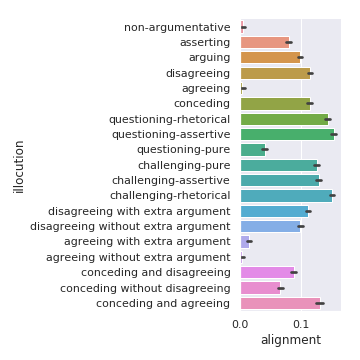
\includegraphics[width=0.45\textwidth]{alignment.png}
\caption{Alignment estimates over IAT discourse acts and combinations of interest. The error bars represent 95\% highest posterior density.}
\end{figure}

\subsection{Alignment Over Comments}

In this preliminary work, we use a simpler method for local alignment at the individual comment-reply level that we found effective. We utilize the author baselines calculated for each LIWC category from the entire dataset. Then, for each message and reply, we calculate the local change in logit space from the baseline to the observed usage rate, based on the binary criterion of whether the original message contained a word from the category. Formally, let the LIWC categories used in the first message be $\mathbb{C}_a$. For a LIWC category $c$, given the baseline logit space probability $\eta^{(c)}$ of the replier, and the observed usage rate $r$ of words from category $c$ in the reply, we calculate the alignment score as

\begin{equation*}
    s^{(c)} = 
    \begin{cases}
        \text{logit}(r) - \eta^{(c)} & c \in \mathbb{C}_a \\
        0 & \text{otherwise}
    \end{cases}
\end{equation*}

\vspace{6pt}

\noindent
We clip these values to be in the range $[-5, 5]$ to avoid infinite values and floor effects - for example where the reply does not contain a word from $c$. This range is large enough to cover the size of alignment effects we observed. Following this calculation method we end up with an $11$-dimensional vector of alignments over each LIWC category for each reply.

\subsection{Detecting Argumentative Discourse Acts}

To investigate our second preliminary research question we perform logistic regression for each annotated comment and each discourse act. Our baseline is a bag of GloVe vectors \cite{PenningtonSM14}. We use the 25-dimensional vectors trained on 27 billion tokens from a Twitter corpus. We concatenate the 11-dimensional alignment score vector to the bag of GloVe representation and look for an increase in performance. We randomly split the dataset into $600$ training data points, and $200$ for testing. We implement logistic regression with Scikit-learn \cite{Pedregosa11} and use the LBFGS solver. We set the maximum number of iterations to $10,000$ to allow enough exploration time. Because this is not a deterministic algorithm, we take the mean performance of 20 runs over different random seeds as the final result. As we are concerned with detection, and because the labels in each class are very imbalanced, our evaluation metric is ROC AUC.

\begin{figure}[t]
\centering
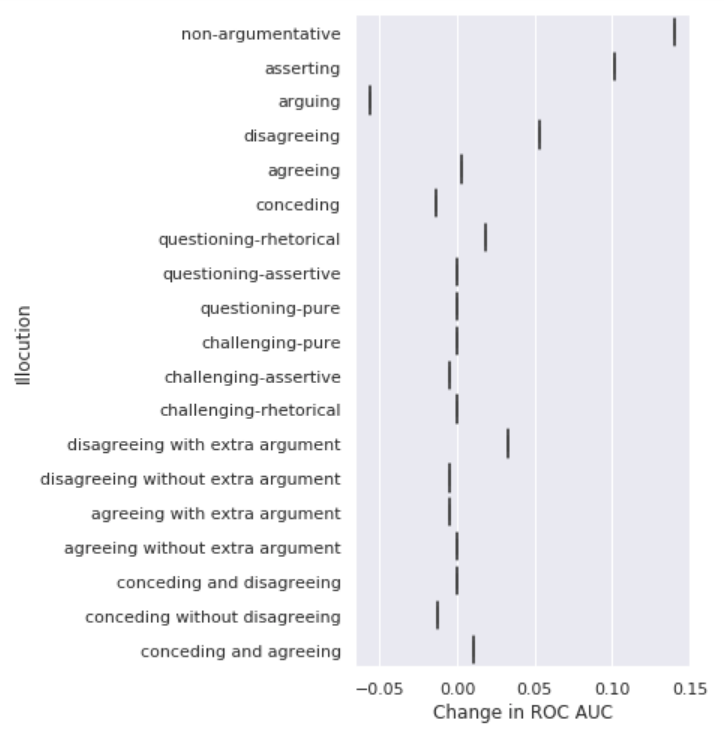
\includegraphics[width=0.45\textwidth]{diff.png}
\caption{ROC AUC Performance change from bag of GloVe vectors due to adding alignment features.}
\end{figure}

\section{Results and Discussion}

All data and code to reproduce these results are available on Github.\footnote{\hyperlink{https://github.com/IKMLab/argalign1}{https://github.com/IKMLab/argalign1}}

\subsection{Alignment and Discourse Acts}

Figure 6 shows the alignment estimates over our annotated discourse acts. Due the limitations of our data we limit our preliminary research question to whether these differences are significant. We conducted pairwise t-tests for the significance of the difference between the means of our alignment estimates for each discourse act. A clear majority were significant ($p >> 0.05$), with only $6.4\%$ ($22/342$) insignificant. We therefore answer our first research question positively.

\subsection{Detecting Discourse Acts}

Figure 7 shows the change in ROC AUC of our logistic regression model with alignment features as compared to the baseline. In general alignment features are useful, with the net change over all discourse acts being positive. We therefore answer our second research question in the affirmative. However, arguing has taken an unexpected step backwards that requires further explanation. It could be a result of overfitting due to the small size of our dataset.

\begin{figure}[t]
\centering
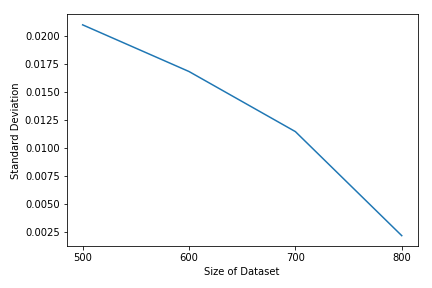
\includegraphics[width=0.45\textwidth]{std.png}
\caption{Mean of the standard deviation of parameter estimates as a function of dataset size. For each dataset size we fit the model 10 times with a different random seed.}
\end{figure}

\section{Reliability}

Due to the limitations of our study we asked the question: how reliable are the alignment estimates presented here? We expect noise to come from three sources: (1) the small size of our dataset; (2) using a non-deterministic optimization algorithm; (3) only having one annotator. We are unable to address (3) in the present work. However we investigated (1) and (2) by fitting our model 10 times with different random seeds for different dataset sizes (500, 600, 700, and 800 data points) and calculating the standard deviation in the estimated parameter means across the 10 runs. The results are given in Figure 8. We can see that by 800 data points the mean of the standard deviation has reduced significantly to around $0.002$. Thus in the aggregate the parameters estimates appear to be converging already - although parameters with few data points still show larger variance. We clearly need more data for lower frequency discourse acts.

\section{Conclusion and Future Work}

We have reported what are likely to be robust results showing significant difference among alignment effects over argumentative discourse acts in a below the line comments genre. Comment level alignment features were shown to be useful for detecting argumentative discourse acts in the aggregate. Our study is limited by a small dataset, which is particularly felt for low frequency discourse acts, and an annotation scheme lacking multiple annotators. Therefore our immediate future work includes expanding our dataset and acquiring multiple annotations. We also plan to make our investigations more robust by including a cross-linguistic comparison with Mandarin data.

Although these results are not robust enough to draw more interesting conclusions about the observed patterns, we make one suggestive observation. Alignment appears higher for discourse acts that involve arguing. \textit{Non-argumentative}, \textit{Agreeing}, and \textit{Pure Questioning} show no alignment effects. In general, \textit{Arguing} and \textit{Disagreeing} increase alignment. There is support in the previous literature for a view of  alignment as modulated by engagement \cite{NiederhofferP02}. Our genre can be characterized as a clash of opinions. If engaging in debate is modulating alignment it would not be surprising if alignment effects were higher over argumentative discourse acts. We leave a thorough treatment of this question to future work.

We note that our agreement and disagreement estimates are at odds with previous work on body and head movement accommodation that showed alignment \textit{decrease} with disagreement \cite{PaxtonD13, DuranF17}. There are some considerations that may account for this discrepancy. Previous work \cite{DoyleF16} showed that alignment was less pronounced in telephone than online textual conversation (Twitter). It was hypothesized that in the textual genre there is time to review the original message when composing a reply. There may also be time to reflect and choose a communication strategy. In face-to-face argumentation, on the other hand, one is forced to react in the moment, with far less time to prepare a considered response. Our tentative results appear to support a view alignment as modulated by \textit{communication strategy} \cite{FusaroliBORRFT12}.

We also need to apply our methods to existing datasets for comparison. In particular the US 2016 Election Reddit corpus \cite{VisserKDKBR19} is already annotated with IAT discourse acts. The IAC should also be used to further investigate the relationship between alignment and disagreement, particularly as our finding appears to contradict previous results.

Our methods, particularly the calculation of local alignment in replying comments, can be sharpened, especially as the volume of data grows. We also note that in our dataset repliers often directly quote large portions of text in the original message. This may skew alignment calculations in these instances. We will apply a preprocessing step in future to control for this. Another peculiar feature of our genre is that comments are often directed to the broader audience. IAC is annotated with this aspect, and it will be important to investigate how this affects alignment. It may be worthwhile investigating methods that consider a broader context than the immediate message and reply. We also need to consider alignment over words as well as categories, particular as previous research showed alignment over words to be a more primary phenomenon \cite{DoyleF16}.


Other phenomenon have been proposed to modulate alignment in argumentation. It has been suggested that arguing a minority position may be accompanied by an increased need for persuasiveness \cite{PennebakerMN03} (and therefore an increased usage of ``causation'' words). Argumentation schemes may also prove to modulate alignment. An argument from authority, for example as an eyewitness, could require a communicative strategy that sounds authoritative - having the power of knowledge. Previous results showed that power does not align but is aligned to. That would lead to the hypothesis that such an argument scheme should be correlated with a smaller or negative alignment effect. Modeling argument schemes directly may therefore help to improve the accuracy of argumentative alignment estimates.

\section*{Acknowledgements}

We would like to thank the reviewers for their helpful comments.

\bibliography{acl2019}
\bibliographystyle{acl_natbib}

\end{document}
